%% ink2midi_ieee.tex
%% IEEE Conference Paper: Ink2MIDI - Deep Learning Pipeline for Handwritten Optical Music Recognition
%% Compile with: pdflatex ink2midi_ieee.tex (twice) ; bibtex if using .bib
%% Template: IEEEtran v1.8b conference mode

\documentclass[conference]{IEEEtran}
\IEEEoverridecommandlockouts

\usepackage{cite}
\usepackage{amsmath,amssymb,amsfonts}
\usepackage{algorithmic}
\usepackage{graphicx}
\usepackage{textcomp}
\usepackage{xcolor}
\usepackage{booktabs}
\usepackage{url}
\usepackage{hyperref}
\hypersetup{
    colorlinks=true,
    linkcolor=black,
    citecolor=black,
    urlcolor=blue
}

\def\BibTeX{{\rm B\kern-.05em{\sc i\kern-.025em b}\kern-.08em
    T\kern-.1667em\lower.7ex\hbox{E}\kern-.125emX}}

\begin{document}

\title{Ink2MIDI: An End-to-End Deep Learning Pipeline for\\Handwritten Optical Music Recognition Using\\YOLOv8 Detection and Graph Attention Networks}

\author{
\IEEEauthorblockN{Ojasvi Poonia}
\IEEEauthorblockA{\textit{M.\ S.\ Ramaiah Institute of Technology}\\
Bangalore, Karnataka, India \\
i.ojasvipoonia@gmail.com}
}

\maketitle

\begin{abstract}
Optical Music Recognition (OMR) for handwritten scores remains a challenging
problem because of writer variability, ink artefacts, and the dense, structurally
constrained layout of musical notation. Existing systems typically address
either symbol localisation or symbol classification in isolation and rarely
deliver an end-to-end output that a musician can play. We present
\textit{Ink2MIDI}, a complete pipeline that converts a single image of a
handwritten music score into a playable MIDI file. The system combines (i) a
YOLOv8-based detector trained with two-phase transfer learning -- pretrained on
the synthetic DeepScores~V2 corpus and fine-tuned on the handwritten
MUSCIMA++ dataset under a writer-disjoint protocol; (ii) a Graph Attention
Network (GAT) operating on a $k$-nearest-neighbour graph of the detected
primitives to recover their structural relationships; and (iii) a rule-based
sequencing module that performs staff-line analysis, clef-aware pitch
resolution, rhythm decoding, and MIDI export via \texttt{music21}. On the
writer-disjoint MUSCIMA++ test split the detector achieves a mAP@0.5 of
\textbf{0.630} (mAP@0.5:0.95 = 0.371) over 26 musical primitive classes.
The pipeline is fully open-source and reproducible, and to the best of our
knowledge is one of the few publicly documented systems that integrates
modern object detection, graph-based relationship parsing, and symbolic
music export in a single repository.
\end{abstract}

\begin{IEEEkeywords}
optical music recognition, handwritten document analysis, object detection,
graph neural networks, graph attention networks, transfer learning,
MUSCIMA++, MIDI, deep learning
\end{IEEEkeywords}

%==============================================================================
\section{Introduction}
%==============================================================================
Music notation is a centuries-old visual language whose digitisation enables
search, analysis, performance, and preservation of an enormous body of
historical and contemporary works. While engraved (typeset) scores can be
processed with high accuracy by commercial OMR systems, recognising
\emph{handwritten} scores remains a substantially harder problem
\cite{calvo2020understanding,shatri2020optical}. The variability of personal
handwriting, deteriorating ink, skewed staves, and the
two-dimensional grammar of music notation together make handwritten OMR an
open research challenge.

Most OMR research separates the problem into staged sub-tasks --- staff-line
removal, primitive detection, classification, and symbolic reconstruction
\cite{rebelo2012optical} --- and the majority of recent learning-based work
\cite{baro2019handwritten,pacha2018handwritten} addresses only the
\emph{detection} or \emph{classification} stage. Comparatively few open
end-to-end pipelines exist that take a raw scanned page and produce a playable
MIDI file. This gap limits both reproducibility and downstream
musicological use.

\textbf{Contributions.} This paper presents Ink2MIDI, an open end-to-end OMR
pipeline for handwritten scores. Our contributions are:
\begin{enumerate}
    \item A reproducible \textbf{two-phase transfer-learning protocol} for
    YOLOv8s, pretrained on the large synthetic DeepScores~V2 corpus and
    fine-tuned on MUSCIMA++ with a strict \textbf{writer-disjoint}
    train/validation/test split, giving mAP@0.5 = 0.630 across 26 primitive
    classes.
    \item A \textbf{Graph Attention Network} for relationship parsing that
    operates on a $k$-nearest-neighbour spatial graph of detected primitives
    with hand-engineered geometric edge features (relative displacement,
    Euclidean distance, angle, scale ratio).
    \item A \textbf{music-aware sequencing module} that performs Hough-based
    staff-line analysis, clef-aware pitch mapping, rhythm decoding from
    notehead/beam/flag/dot evidence, and \texttt{music21}-driven MIDI export.
    \item A \textbf{fully open-source, reproducible implementation} with
    automated dataset download, configuration files, training scripts, and an
    inference entry point that produces a MIDI file from a single image.
\end{enumerate}

The remainder of the paper is organised as follows. Section~\ref{sec:related}
surveys related work. Section~\ref{sec:method} describes the pipeline in
detail. Section~\ref{sec:experiments} reports the experimental setup and
Section~\ref{sec:results} the results. Section~\ref{sec:discussion} discusses
limitations and ethical considerations, and Section~\ref{sec:conclusion}
concludes.

%==============================================================================
\section{Related Work}\label{sec:related}
%==============================================================================
\subsection{Optical Music Recognition}
Classical OMR pipelines decompose the task into staff-line removal, primitive
segmentation, classification, and reconstruction
\cite{rebelo2012optical,calvo2020understanding}. Modern learning-based
approaches have moved towards end-to-end recognition. Calvo-Zaragoza
\textit{et al.}~\cite{calvo2018camera} treat single-staff transcription as an
image-to-sequence problem with CNN--RNN--CTC architectures. Bar\'o
\textit{et al.}~\cite{baro2019handwritten} explore sequence models for
handwritten staves. Shatri and Fazekas~\cite{shatri2020optical} provide a
recent survey, noting that full-page handwritten OMR with playable output is
still an open problem.

\subsection{Object Detection for Music Notation}
Pacha \textit{et al.}~\cite{pacha2018handwritten} were among the first to apply
deep object detectors (Faster R-CNN, RetinaNet) to MUSCIMA++. Tuggener
\textit{et al.}~\cite{tuggener2018deepscores,tuggener2024deepscores2} introduced
the DeepScores corpus of synthetic engraved scores designed specifically for
detector pretraining. We build on this line of work by adopting YOLOv8
\cite{jocher2023yolov8}, a modern anchor-free detector, and using
DeepScores~V2 as a pretraining source for a downstream MUSCIMA++ fine-tune.

\subsection{Graph Neural Networks for Document Structure}
Music notation is naturally described as a graph: noteheads attach to stems,
stems connect to beams and flags, accidentals modify the following notehead,
and so on. Graph neural networks have proven effective at recovering such
structural relations in documents
\cite{kipf2017semi,velickovic2018graph,riba2020table}. We use a Graph
Attention Network~\cite{velickovic2018graph} to predict whether each candidate
edge in a $k$-NN graph of detected primitives corresponds to a real
musical relationship (e.g.\ ``stem-of'', ``beamed-with'').

\subsection{Symbolic Music Representation}
Once primitives and their relations are known, a symbolic representation must
be assembled and exported. We rely on \texttt{music21}~\cite{cuthbert2010music21}
for score construction and MIDI serialisation; the same library underpins many
musicological systems and is therefore a natural deployment target.

%==============================================================================
\section{Methodology}\label{sec:method}
%==============================================================================
Figure~\ref{fig:pipeline} shows the four stages of the pipeline. The remainder
of this section describes each stage.

\begin{figure*}[t]
\centering
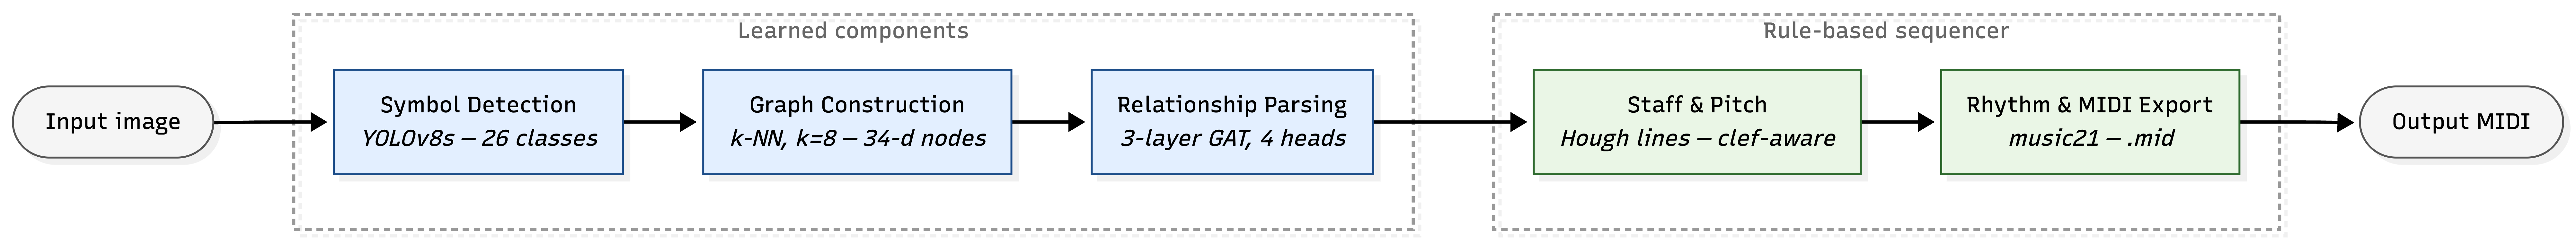
\includegraphics[width=0.95\textwidth]{pipeline.png}
\caption{Ink2MIDI pipeline overview. A YOLOv8s detector localises 26 classes
of musical primitives; a $k$-NN spatial graph is built over the detections,
and a 3-layer Graph Attention Network classifies each candidate edge as a
musical relationship. A rule-based sequencer then performs Hough-based
staff-line analysis, clef-aware pitch resolution, rhythm decoding, and MIDI
export through \texttt{music21}.}
\label{fig:pipeline}
\end{figure*}

\subsection{Datasets and Preparation}\label{sec:data}
We use three publicly available corpora:
\begin{itemize}
    \item \textbf{MUSCIMA++ v2}~\cite{hajic2017muscima} -- 140 handwritten
    pages from 50 writers with 91{,}254 annotated symbols. Used for fine-tuning
    the detector and for training the GAT.
    \item \textbf{CVC-MUSCIMA}~\cite{fornes2012cvcmuscima} -- the source
    images underlying MUSCIMA++.
    \item \textbf{DeepScores~V2}~\cite{tuggener2024deepscores2} -- 1{,}714
    digitally engraved pages with dense annotations, used for detector
    pretraining.
\end{itemize}
We map MUSCIMA++ classes to a unified 26-class label set covering noteheads
(filled, half, whole), stems, beams, flags (eighth/sixteenth, up/down), rests
(whole through sixteenth), accidentals (sharp, flat, natural, double sharp),
clefs (treble, bass, alto), time-signature digits, bar lines, dots, and
ties/slurs. Annotations are converted to YOLO format
($\langle\text{class},x_c,y_c,w,h\rangle$, normalised). The MUSCIMA++ split
is \textbf{writer-disjoint}: writers~1--35 train, 36--42 validate, 43--50
test. This protocol prevents writer-identity leakage and is essential for
honest generalisation claims; many earlier OMR results inadvertently use
random splits in which the same writer appears across folds.

\subsection{Symbol Detection}\label{sec:detection}
We adopt YOLOv8s~\cite{jocher2023yolov8} (11.2M parameters, 28.5 GFLOPs) as the
primitive detector. Training proceeds in two phases:
\begin{enumerate}
    \item \emph{Pretrain on DeepScores~V2.} Initialised from COCO weights;
    SGD (momentum 0.937, weight decay $5\times 10^{-4}$); image size
    $640\times 640$; batch size 16; up to 100 epochs with patience-30 early
    stopping. Mosaic is reduced to 0.5 and random rotation capped at $3^\circ$
    because larger rotations and flips invalidate music semantics
    (vertical flip swaps stem direction; horizontal flip mirrors clefs).
    \item \emph{Fine-tune on MUSCIMA++.} Initialised from the Phase-1
    checkpoint; learning rate $10^{-3}$; batch size 8; up to 150 epochs.
\end{enumerate}
Inference uses a confidence threshold of 0.3 and NMS IoU 0.45. A music-aware
post-processing pass discards geometrically implausible detections (e.g.\
isolated stems with no nearby notehead).

\subsection{Graph Construction and Relationship Parsing}\label{sec:gat}
The detected primitives form the nodes of a graph $G=(V,E)$. For each node
$v_i$ we construct a 34-dimensional feature vector consisting of a 26-d
one-hot class encoding and 8 geometric attributes derived from the bounding
box (centre coordinates, width, height, area, aspect ratio, and two
local-context terms). Edges are formed by $k$-nearest-neighbour connectivity
in image space with $k=8$ and a maximum radius of 200~px to avoid spurious
long-range edges.

For each candidate edge $(v_i,v_j)$ we compute a 5-dimensional feature vector
\[
e_{ij} = \big[\,\Delta x,\ \Delta y,\ \lVert\Delta\rVert_2,\ \theta_{ij},\
\log(s_i/s_j)\,\big]
\]
where $\Delta x,\Delta y$ are the centre offsets, $\theta_{ij}$ is the edge
orientation, and $s_i,s_j$ are bounding-box scales. The relationship parser is
a 3-layer Graph Attention Network~\cite{velickovic2018graph} with 4 attention
heads and a 128-dimensional hidden state, optimised with AdamW
($\text{lr}=10^{-3}$, weight decay $10^{-4}$) and cosine warm restarts
($T_0=20$). Each edge is classified as relation/no-relation with a sigmoid
output; predicted relations are then aggregated via a union--find pass to form
high-level note objects (notehead $\cup$ stem $\cup$ beams/flags $\cup$ dots).
A GCN baseline~\cite{kipf2017semi} is provided for ablation.

\subsection{Staff Analysis, Pitch and Rhythm Resolution}
\label{sec:sequencing}
\textbf{Staff lines.} The Hough transform is applied to the binarised image to
recover the five-line staff template. Per-system staff height $h_s$ defines
the vertical reference for pitch.

\textbf{Pitch.} For each notehead we compute its vertical position relative to
the nearest staff and convert it to a diatonic step. The active clef
(detected as a primitive) determines the absolute MIDI pitch via the standard
clef-to-line mapping, with key-signature accidentals (sharp/flat near the
clef) and inline accidentals applied within their measure of validity.

\textbf{Rhythm.} The duration of a notehead is decided by combining its class
(filled, half, whole) with the count of attached beams and flags and the
presence of dots. Rests are decoded directly from their detected class.

\textbf{Score assembly and MIDI export.} The resulting note and rest events
are inserted into a \texttt{music21} \texttt{Score} object, voiced per staff,
and serialised to a Standard MIDI File at a default tempo of 120~BPM.

%==============================================================================
\section{Experimental Setup}\label{sec:experiments}
%==============================================================================
\subsection{Hardware and Software}
All experiments were carried out on a workstation with an
\textbf{NVIDIA RTX 3070 Ti} GPU (8~GB VRAM, CUDA 12.2). The implementation
uses Python 3.11, PyTorch~2.2 with FP16 automatic mixed precision and
cuDNN benchmark mode, Ultralytics YOLOv8 for detection, PyTorch
Geometric for graph learning, and \texttt{music21} for symbolic export.

\subsection{Reproducibility}
Random seeds are fixed across NumPy, PyTorch, and CUDA. All hyper-parameters
are stored in versioned YAML files (OmegaConf), and dataset preparation is
fully scripted. The repository, configurations, and training scripts are
publicly released to allow exact reproduction of the reported numbers (see
Sec.~\ref{sec:availability}).

\subsection{Evaluation Protocol}
The detector is evaluated on the writer-disjoint MUSCIMA++ test split using
the standard COCO-style mAP@0.5 and mAP@0.5:0.95 metrics, alongside
class-wise precision and recall. Where reported in this paper, all numbers
are computed on writers \emph{never seen} during training. The GAT and
end-to-end MIDI evaluation are reported separately in
Sec.~\ref{sec:results}.

%==============================================================================
\section{Results}\label{sec:results}
%==============================================================================
\subsection{Symbol Detection}
Table~\ref{tab:overall} reports the overall detector performance on the
writer-disjoint test set; Table~\ref{tab:perclass} gives a per-class
breakdown for the 16 most frequent classes.

\begin{table}[h]
\caption{Overall detection performance on the writer-disjoint MUSCIMA++ test
split (YOLOv8s, two-phase transfer learning).}
\label{tab:overall}
\centering
\begin{tabular}{lc}
\toprule
\textbf{Metric} & \textbf{Value} \\
\midrule
mAP@0.5         & 0.630 \\
mAP@0.5:0.95    & 0.371 \\
Precision       & 0.705 \\
Recall          & 0.518 \\
\bottomrule
\end{tabular}
\end{table}

\begin{table}[h]
\caption{Per-class detection results (selected high-frequency classes).}
\label{tab:perclass}
\centering
\small
\begin{tabular}{lccccc}
\toprule
\textbf{Class} & \textbf{N} & \textbf{P} & \textbf{R} & \textbf{mAP@.5} & \textbf{mAP@.5:.95} \\
\midrule
notehead\_filled  & 2982 & 0.847 & 0.698 & 0.802 & 0.355 \\
notehead\_half    &  210 & 0.721 & 0.629 & 0.703 & 0.320 \\
notehead\_whole   &   24 & 0.650 & 0.542 & 0.688 & 0.443 \\
stem              & 2929 & 0.812 & 0.167 & 0.488 & 0.195 \\
beam              &  919 & 0.828 & 0.560 & 0.723 & 0.436 \\
flag\_eighth\_up  &  152 & 0.839 & 0.513 & 0.683 & 0.258 \\
flag\_eighth\_dn  &  167 & 0.872 & 0.695 & 0.801 & 0.402 \\
rest\_quarter     &  115 & 0.805 & 0.896 & 0.924 & 0.590 \\
rest\_eighth      &  163 & 0.937 & 0.724 & 0.850 & 0.537 \\
sharp             &  295 & 0.890 & 0.661 & 0.785 & 0.428 \\
flat              &  161 & 0.821 & 0.627 & 0.749 & 0.381 \\
treble\_clef      &   59 & 0.967 & 0.983 & 0.991 & 0.769 \\
bass\_clef        &   38 & 0.972 & 0.921 & 0.958 & 0.735 \\
alto\_clef        &   27 & 0.960 & 0.889 & 0.942 & 0.689 \\
tie\_slur         &  431 & 0.889 & 0.777 & 0.859 & 0.553 \\
bar\_line         &  445 & 0.793 & 0.535 & 0.654 & 0.317 \\
\bottomrule
\end{tabular}
\end{table}

\textbf{Observations.}
(i)~Clefs are recognised almost perfectly (mAP@0.5 $> 0.94$ for all three
clefs), which is critical because misidentifying a clef shifts every
subsequent pitch.
(ii)~Rests (especially quarter and eighth) achieve the highest mAP@0.5:0.95
scores, reflecting their compact, distinctive shapes.
(iii)~The most challenging class is \texttt{stem}, with a recall of only
0.167 despite high precision (0.812). Stems are long, thin, and frequently
overlap with beams; the YOLO IoU criterion is unforgiving for elongated
shapes whose centre coordinates may be predicted accurately but whose
extent is under-estimated. Improving stem recall is one of the principal
levers for end-to-end accuracy and is discussed in
Sec.~\ref{sec:discussion}.

\subsection{Graph Attention Network}
\textit{[Reserved for the GAT relationship-parsing results to be inserted
after the next training run. Recommended metrics: edge-level precision /
recall / F1 and AUROC on the writer-disjoint test set, plus an ablation
against the GCN baseline implemented in
\texttt{src/omr/relationship/gcn\_model.py}.]}

\subsection{End-to-End MIDI Evaluation}
\textit{[Reserved for end-to-end MIDI accuracy on a held-out subset.
Recommended metrics: note-level F1 (pitch-only and pitch+onset+duration),
plus a small-scale qualitative listening study.]}

\subsection{Training Time}
\begin{table}[h]
\caption{Wall-clock training time on a single NVIDIA RTX~3070~Ti.}
\label{tab:time}
\centering
\begin{tabular}{lc}
\toprule
\textbf{Phase} & \textbf{Duration} \\
\midrule
YOLOv8 pretrain (DeepScores, 100 epochs)      & $\sim$1--2 h \\
YOLOv8 fine-tune (MUSCIMA++, 150 epochs)      & $\sim$15--30 min \\
GAT training (200 epochs, early stopping)      & $\sim$5--10 min \\
\midrule
Total                                          & $\sim$1.5--2.5 h \\
\bottomrule
\end{tabular}
\end{table}

%==============================================================================
\section{Discussion, Limitations and Ethics}\label{sec:discussion}
%==============================================================================
\subsection{What Works Well}
The two-phase transfer-learning protocol delivers strong detection on a
small handwritten corpus by leveraging the much larger synthetic
DeepScores~V2 dataset. The decision to use a writer-disjoint split
exposes the difficulty of the problem honestly and yields results that
should generalise to truly unseen handwriting.

\subsection{Limitations}
We identify the following limitations that we believe are important to
report transparently:
\begin{itemize}
    \item \textbf{Stem recall.} As noted above, stem detection has low recall
    under the strict IoU criterion. Because stems anchor most rhythmic
    decoding, this is the largest single source of downstream error.
    Strategies under investigation include line-aware loss formulations and
    explicit stem post-processing seeded by detected noteheads.
    \item \textbf{Class coverage.} The current label set covers 26 primitive
    classes. Less frequent symbols (ornaments, dynamics, articulation marks,
    text) are not yet handled; their absence does not invalidate the
    pipeline but limits musical fidelity for ornate scores.
    \item \textbf{Polyphony and voicing.} The sequencer assumes a single
    voice per staff. Multi-voice handwritten music with shared stems
    requires additional voicing logic.
    \item \textbf{Dataset size.} MUSCIMA++ provides 140 pages from 50
    writers. While writer-disjoint evaluation mitigates leakage, broader
    generalisation will require larger and more diverse handwritten corpora.
    \item \textbf{End-to-end MIDI accuracy.} Quantitative end-to-end MIDI
    metrics are not yet reported; we explicitly mark them as future work
    rather than estimate them.
\end{itemize}

\subsection{Ethical Considerations}
All datasets used in this work (MUSCIMA++, CVC-MUSCIMA, DeepScores~V2) are
publicly released for research use under their respective licences, and we
use them in accordance with those terms. No personal data beyond the
identifiers of the original writers (already published with the dataset)
is processed, and no attempt is made to identify or profile individual
writers; writer IDs are used solely to construct disjoint evaluation
splits. The pipeline does not generate music attributed to any third
party; it transcribes input scores supplied by the user. Users should
ensure they hold the necessary rights to the scores they transcribe.

\subsection{Reproducibility and Code Availability}\label{sec:availability}
The complete source code, configuration files, training scripts and
inference entry points are released as open source under the MIT licence at
\url{https://github.com/Ojasvi-Poonia/ink2midi}. Dataset download is
automated. All hyper-parameters, splits, and seeds reported in this paper
are tracked in version control.

%==============================================================================
\section{Conclusion and Future Work}\label{sec:conclusion}
%==============================================================================
We presented Ink2MIDI, a reproducible end-to-end pipeline that turns a
single image of a handwritten music score into a playable MIDI file. The
system combines YOLOv8 detection with a two-phase transfer-learning
protocol from synthetic to handwritten data, a Graph Attention Network for
structural relationship parsing on a $k$-NN graph of detected primitives,
and a music-theory-aware sequencer that exports through \texttt{music21}.
Under a strict writer-disjoint protocol on MUSCIMA++ the detector reaches
mAP@0.5 = 0.630 over 26 musical primitive classes.

Future work targets three axes: (i) improving stem recall through
line-aware detection losses; (ii) extending the label set to ornaments,
dynamics and articulations; and (iii) reporting full end-to-end MIDI
metrics via a held-out evaluation set, including a small listening study
with trained musicians.

%==============================================================================
\section*{Acknowledgements}
%==============================================================================
The author thanks the maintainers of MUSCIMA++, CVC-MUSCIMA and DeepScores~V2
for releasing their data, and the developers of YOLOv8, PyTorch Geometric and
\texttt{music21} for their open-source tools.

%==============================================================================
% References
%==============================================================================
\begin{thebibliography}{00}

\bibitem{calvo2020understanding}
J.~Calvo-Zaragoza, J.~Hajic Jr., and A.~Pacha,
``Understanding Optical Music Recognition,''
\emph{ACM Computing Surveys}, vol.~53, no.~4, pp.~1--35, 2020.

\bibitem{shatri2020optical}
E.~Shatri and G.~Fazekas,
``Optical Music Recognition: State of the Art and Major Challenges,''
in \emph{Proc.\ International Conference on Technologies for Music Notation
and Representation (TENOR)}, 2020.

\bibitem{rebelo2012optical}
A.~Rebelo, I.~Fujinaga, F.~Paszkiewicz, A.~R.~S.~Marcal, C.~Guedes, and
J.~S.~Cardoso,
``Optical music recognition: state-of-the-art and open issues,''
\emph{International Journal of Multimedia Information Retrieval},
vol.~1, no.~3, pp.~173--190, 2012.

\bibitem{baro2019handwritten}
A.~Bar\'o, P.~Riba, J.~Calvo-Zaragoza, and A.~Forn\'es,
``From optical music recognition to handwritten music recognition: A baseline,''
\emph{Pattern Recognition Letters}, vol.~123, pp.~1--8, 2019.

\bibitem{pacha2018handwritten}
A.~Pacha, J.~Hajic Jr., and J.~Calvo-Zaragoza,
``A baseline for general music object detection with deep learning,''
\emph{Applied Sciences}, vol.~8, no.~9, p.~1488, 2018.

\bibitem{calvo2018camera}
J.~Calvo-Zaragoza, J.~J.~Valero-Mas, and A.~Pertusa,
``End-to-end optical music recognition using neural networks,''
in \emph{Proc.\ International Society for Music Information Retrieval
Conference (ISMIR)}, 2017.

\bibitem{tuggener2018deepscores}
L.~Tuggener, I.~Elezi, J.~Schmidhuber, M.~Pelillo, and T.~Stadelmann,
``DeepScores -- A dataset for segmentation, detection and classification of
tiny objects,''
in \emph{Proc.\ International Conference on Pattern Recognition (ICPR)}, 2018.

\bibitem{tuggener2024deepscores2}
L.~Tuggener, Y.~Satyawan, A.~Pacha, J.~Schmidhuber, and T.~Stadelmann,
``The DeepScoresV2 dataset and benchmark for music object detection,''
in \emph{Proc.\ International Conference on Pattern Recognition (ICPR)}, 2020.
% Update with the precise venue/year you wish to cite

\bibitem{jocher2023yolov8}
G.~Jocher, A.~Chaurasia, and J.~Qiu,
``Ultralytics YOLOv8,'' 2023. [Online]. Available:
\url{https://github.com/ultralytics/ultralytics}

\bibitem{kipf2017semi}
T.~N.~Kipf and M.~Welling,
``Semi-supervised classification with graph convolutional networks,''
in \emph{Proc.\ International Conference on Learning Representations (ICLR)}, 2017.

\bibitem{velickovic2018graph}
P.~Veli\v{c}kovi\'c, G.~Cucurull, A.~Casanova, A.~Romero, P.~Li\`o, and
Y.~Bengio,
``Graph attention networks,''
in \emph{Proc.\ International Conference on Learning Representations (ICLR)}, 2018.

\bibitem{riba2020table}
P.~Riba, A.~Dutta, L.~Goldmann, A.~Forn\'es, O.~Ramos, and J.~Llad\'os,
``Table detection in invoice documents by graph neural networks,''
in \emph{Proc.\ International Conference on Document Analysis and Recognition
(ICDAR)}, 2019.

\bibitem{cuthbert2010music21}
M.~S.~Cuthbert and C.~Ariza,
``music21: A toolkit for computer-aided musicology and symbolic music data,''
in \emph{Proc.\ International Society for Music Information Retrieval
Conference (ISMIR)}, 2010.

\bibitem{hajic2017muscima}
J.~Hajic Jr.\ and P.~Pecina,
``The MUSCIMA++ dataset for handwritten optical music recognition,''
in \emph{Proc.\ International Conference on Document Analysis and Recognition
(ICDAR)}, 2017.

\bibitem{fornes2012cvcmuscima}
A.~Forn\'es, A.~Dutta, A.~Gordo, and J.~Llad\'os,
``CVC-MUSCIMA: A ground-truth of handwritten music score images for writer
identification and staff removal,''
\emph{International Journal on Document Analysis and Recognition},
vol.~15, no.~3, pp.~243--251, 2012.

\end{thebibliography}

\end{document}
